\begin{pastexam}[label={px:ntu-109-comm-dsa-36}]{臺大電信所 109 學年度（B）第 36--42 題}
（單選；每題 2 分，答錯不倒扣）

For problems 36 to 42, please refer to the following dynamic programming problem.

\begin{center}
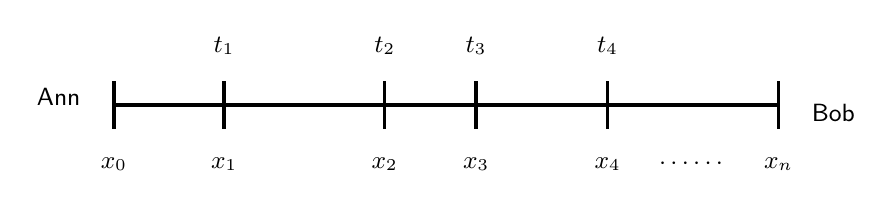
\begin{tikzpicture}[font=\small]
\draw[very thick] (0,0)--(8.44,0);
\draw[very thick] (0.00,-0.3)--(0.00,0.3);
\node at (0.00,-0.75) {$x_0$};
\draw[very thick] (1.40,-0.3)--(1.40,0.3);
\node at (1.40,-0.75) {$x_1$};
\node at (1.40,0.75) {$t_1$};
\draw[very thick] (3.44,-0.3)--(3.44,0.3);
\node at (3.44,-0.75) {$x_2$};
\node at (3.44,0.75) {$t_2$};
\draw[very thick] (4.60,-0.3)--(4.60,0.3);
\node at (4.60,-0.75) {$x_3$};
\node at (4.60,0.75) {$t_3$};
\draw[very thick] (6.27,-0.3)--(6.27,0.3);
\node at (6.27,-0.75) {$x_4$};
\node at (6.27,0.75) {$t_4$};
\draw[very thick] (8.44,-0.3)--(8.44,0.3);
\node at (8.44,-0.75) {$x_n$};
\node at (7.33,-0.75) {$\cdots\cdots$};
\node[left] at (-0.3,0.1) {\textsf{Ann}};
\node[right] at (8.74,-0.1) {\textsf{Bob}};
\end{tikzpicture}
\end{center}

Ann is riding scooter from her home to Bob's home with a constant speed $v$. However, her scooter
can only hold gas for 100kms riding at most. There are a few gas stations along the way at
$x_1,x_2,\ldots,x_n$ distances from her home, but filling up at different stations $x_i$ would take
different time $t_i$. She would start her trip with a full tank of gas, and if she decides to fill
up at a gas station, she needs to fill her entire tank up. Since the riding time is constant
$(x_n/v)$, we only need to consider the time consumed by filling gas. (Assume that the distances
between two consecutive stations are not longer than 100kms. Bob's home is at $x_n$ distances from
Ann's home and the distances between his home and the last station are not longer than 100kms as
well.)

\begin{enumerate}[label=\arabic*., start=36, leftmargin=2.2em]
\item If $s[a]$ indicates the minimum time she has spent on filling gas when she has filled the gas
at $a^{\text{th}}$ station, then
\begin{enumerate}[label=(\Alph*)]
\item $s[a]=\begin{cases}0, & \text{if } a=0\\ \displaystyle\min_{(0\le i\le a-1)\wedge(x_a-x_i\le 100)}(s[i]+t[i]), & \text{otherwise}\end{cases}$
\item $s[a]=\begin{cases}0, & \text{if } a=0\\ \displaystyle\min_{(0\le i\le a-1)\wedge(x_a-x_i\le 100)}(s[i]+t[a]), & \text{otherwise}\end{cases}$
\end{enumerate}
\item If $r[a]$ indicates the minimum time she has spent on filling gas when she arrives at
$a^{\text{th}}$ gas station, then
\begin{enumerate}[label=(\Alph*)]
\item $r[a]=\begin{cases}0, & \text{if } a=0\\ \displaystyle\min_{(0\le i\le a-1)\wedge(x_a-x_i\le 100)}(r[i]+t[i]), & \text{otherwise}\end{cases}$
\item $r[a]=\begin{cases}0, & \text{if } a=0\\ \displaystyle\min_{(0\le i\le a-1)\wedge(x_a-x_i\le 100)}(r[i]+t[a]), & \text{otherwise}\end{cases}$
\end{enumerate}
\end{enumerate}

\begin{center}
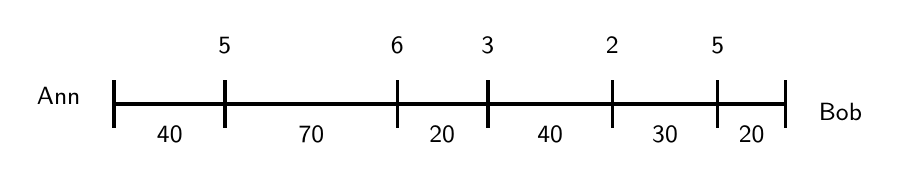
\begin{tikzpicture}[font=\small\sffamily]
\draw[very thick] (0,0)--(8.53,0);
\draw[very thick] (0.00,-0.3)--(0.00,0.3);
\node at (0.71,-0.38) {40};
\draw[very thick] (1.41,-0.3)--(1.41,0.3);
\node at (1.41,0.75) {5};
\node at (2.51,-0.38) {70};
\draw[very thick] (3.60,-0.3)--(3.60,0.3);
\node at (3.60,0.75) {6};
\node at (4.17,-0.38) {20};
\draw[very thick] (4.75,-0.3)--(4.75,0.3);
\node at (4.75,0.75) {3};
\node at (5.54,-0.38) {40};
\draw[very thick] (6.33,-0.3)--(6.33,0.3);
\node at (6.33,0.75) {2};
\node at (7.00,-0.38) {30};
\draw[very thick] (7.67,-0.3)--(7.67,0.3);
\node at (7.67,0.75) {5};
\node at (8.10,-0.38) {20};
\draw[very thick] (8.53,-0.3)--(8.53,0.3);
\node[left] at (-0.3,0.1) {Ann};
\node[right] at (8.83,-0.1) {Bob};
\end{tikzpicture}
\end{center}

According to the figure, solve $s[1],\ldots,s[5]$.

\noindent\begin{tabular}{@{}l@{\quad}l@{\quad}l@{\quad}l@{\quad}l@{}}
38. $s[1]=$ & (A)~0 & (B)~5 & (C)~6 & (D)~40 \\
39. $s[2]=$ & (A)~0 & (B)~5 & (C)~6 & (D)~11 \\
40. $s[3]=$ & (A)~5 & (B)~8 & (C)~11 & (D)~13 \\
41. $s[4]=$ & (A)~8 & (B)~10 & (C)~11 & (D)~13 \\
42. $s[5]=$ & (A)~8 & (B)~10 & (C)~11 & (D)~13
\end{tabular}
\end{pastexam}

\begin{pastsoln}
答案：36 (B)；37 (A)；38 (B) $5$；39 (D) $11$；40 (B) $8$；41 (B) $10$；42 (D) $13$。

原卷第 36 到 42 題共用同一段說明和圖，這裡收成一題。 遞迴式裡的 $t[i]$ 就是說明裡的 $t_i$；
$a = 0$ 代表 Ann 的家（$x_0 = 0$），她出發時油箱是滿的，相當於「在第 $0$ 站加滿、不花時間」，
所以取 $t[0] = 0$。 油箱能騎 $100$ 公里，從第 $i$ 站加滿後能直接騎到第 $a$ 站的條件就是
$x_a - x_i \le 100$。

\textbf{36：$s[a]$ 的遞迴式，選 (B)。} $s[a]$ 是「在第 $a$ 站加了油」時到目前為止的最少加油
時間，所以一定包含這一站的 $t[a]$。 在第 $a$ 站加油之前，上一次加油在某個第 $i$ 站（$i < a$，
$i = 0$ 表示從家裡出發後都沒加過），而且從第 $i$ 站滿油騎到第 $a$ 站不能超過 $100$ 公里。 對
所有可能的 $i$ 取最小（資結書第~18.1.5~節：先看最佳解的最後一步有哪些選擇）：
\[
s[a] = \min_{\substack{0 \le i \le a - 1\\ x_a - x_i \le 100}} \bigl(s[i] + t[a]\bigr), \qquad s[0] = 0 .
\]
最佳子結構：如果在第 $a$ 站加油的最佳方案上一次是在第 $i$ 站加油，那它到第 $i$ 站為止的部分
一定是「在第 $i$ 站加油」的最佳方案，否則換成更好的會讓總時間更少。 (A) 加的是 $t[i]$，
$s[i]$ 已經包含 $t[i]$，等於第 $i$ 站算了兩次，第 $a$ 站卻沒算。

\textbf{37：$r[a]$ 的遞迴式，選 (A)。} $r[a]$ 是「到達第 $a$ 站時」（還沒決定在這站加不加油）
的最少加油時間。 到達第 $a$ 站之前最後一次加油在第 $i$ 站，那次花了 $t[i]$，在那之前到達第
$i$ 站時已花了 $r[i]$，所以
\[
r[a] = \min_{\substack{0 \le i \le a - 1\\ x_a - x_i \le 100}} \bigl(r[i] + t[i]\bigr), \qquad r[0] = 0 .
\]
(B) 加的是還沒發生的 $t[a]$，那是 $s$ 的定義。 兩者的關係是 $s[a] = r[a] + t[a]$。

\textbf{38--42：照圖計算。} 圖上各段距離是 $40, 70, 20, 40, 30, 20$，站上的數字是加油時間。 累加
得各站位置（Bob 家是 $x_6$）：
\begin{center}
\begin{tabular}{ccccccccc}
\toprule
$a$ & 0（家） & 1 & 2 & 3 & 4 & 5 & 6（Bob） \\
\midrule
$x_a$ & 0 & 40 & 110 & 130 & 170 & 200 & 220 \\
$t[a]$ & 0 & 5 & 6 & 3 & 2 & 5 & -- \\
\bottomrule
\end{tabular}
\end{center}
依 $a$ 由小到大算 $s[a]$，每次只考慮距離不超過 $100$ 的前面的站：
\begin{itemize}
\item $s[1]$：$x_1 - x_0 = 40$，只有 $i = 0$：$s[1] = 0 + 5 = 5$。 選 (B)。
\item $s[2]$：$x_2 - x_0 = 110 > 100$ 不行；$x_2 - x_1 = 70$，$i = 1$：$s[2] = 5 + 6 = 11$。
選 (D)。
\item $s[3]$：$x_3 = 130$。 $i = 0$：$130 > 100$ 不行；$i = 1$：$90$，$5 + 3 = 8$；$i = 2$：$20$，
$11 + 3 = 14$。 $s[3] = 8$。 選 (B)。
\item $s[4]$：$x_4 = 170$。 $i = 1$：$130$ 不行；$i = 2$：$60$，$11 + 2 = 13$；$i = 3$：$40$，
$8 + 2 = 10$。 $s[4] = 10$。 選 (B)。
\item $s[5]$：$x_5 = 200$。 $i = 1$：$160$ 不行；$i = 2$：$90$，$11 + 5 = 16$；$i = 3$：$70$，
$8 + 5 = 13$；$i = 4$：$30$，$10 + 5 = 15$。 $s[5] = 13$。 選 (D)。
\end{itemize}

整個問題的答案（題目沒問）：最後一次加油要在離 Bob 家 $100$ 公里以內，也就是第 $3, 4, 5$ 站
（$220 - 110 = 110 > 100$，第 $2$ 站不行），取 $\min(s[3], s[4], s[5]) = 8$：在第 $1$ 站和第 $3$
站加油。 用 $r$ 算也一樣，$r[6] = 8$。 每個 $s[a]$ 最多看 $a$ 個前面的站，$n$ 個站共 $O(n^2)$。
\end{pastsoln}
